% course:       CV
% teacher:      DongHui Wang
% author:       zju_cs / Yi Zhang / 21721190
% mail:         yizhangzc@gmail.com
% data:         2018/5
% environment:  ubuntu 16.04 / texlive-full / texlive-xetex      
% compiler:     xelatex / bibtex

\documentclass[a4paper]{article}

\usepackage{ctex}           % support chinese
\usepackage{geometry}       % setting margin
\usepackage{setspace}       % setting space
\usepackage{graphicx}       % support insert iamge
\usepackage{subcaption}


\title{deep learning for localization}
\date{2018-05}
\author{张毅\hspace{1em}21721190}

\geometry{left=3cm,right=3cm,top=2.5cm,bottom=2.5cm}

\begin{document}

    \pagenumbering{gobble}
    
    \begin{center}
        \doublespacing
        
        \Large \textbf{Deep learning for localization}

        \normalsize 姓名:张毅 \qquad 学号:21721190 \qquad 日期:2018-5
    \end{center}

    \section{问题描述}

    在CUBdataset数据集上训练模型执行localization任务,框出小鸟位置。

    数据集: CUBData(由助教提供),按照要求,随机选取80\%作为训练数据,其余20\%作为测试数据。

    \section{方法及原理}

    实验中采用了vgg16进行fine-tuning(将在ImageNet上预训练好的vgg16最后一层替换为4个输出单元)进行回归预测,代码已经上传到github仓库(yizhangzc/course),本次实验代码放置在localization文件夹下,运行方式及运行环境见README.md。

    注:课件示例使用了ResNet18,因为在网上没能找到训练好的ResNet18的checkpoint文件来进行fine-tuning,所以本次实验选择了vgg16进行。

    \section{实验结果}

    因为数据集较大,训练很慢,训练只迭代了10000次,模型并未到达最佳效果,loss仍然有下降趋势,但是已经到达可接受范围。结果如下:

        \begin{figure}[htbp]
            \centering
            \begin{subfigure}[b]{0.7\textwidth}
                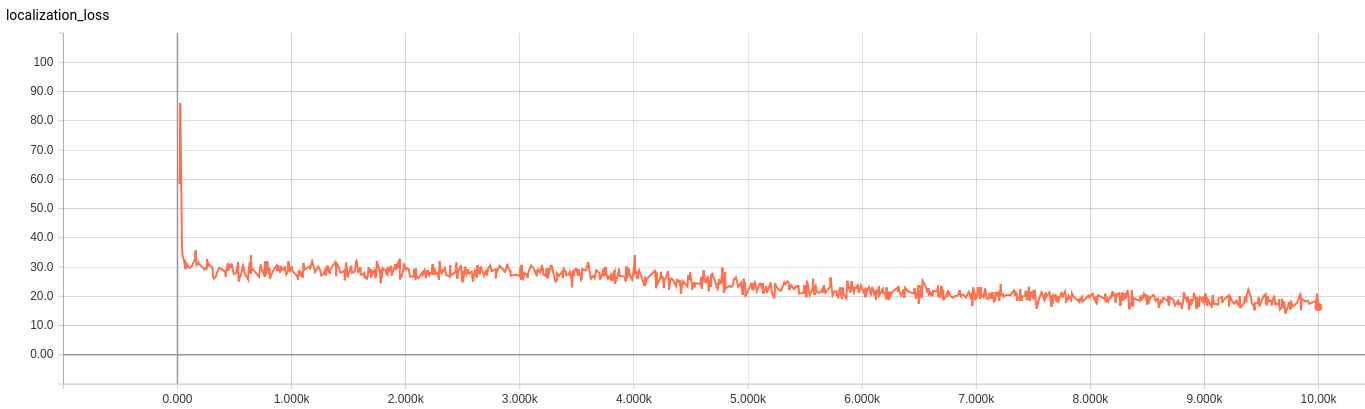
\includegraphics[width=\textwidth]{./images/loss_localization.png}
                \caption{loss下降过程}
            \end{subfigure}
            \begin{subfigure}[b]{0.7\textwidth}
                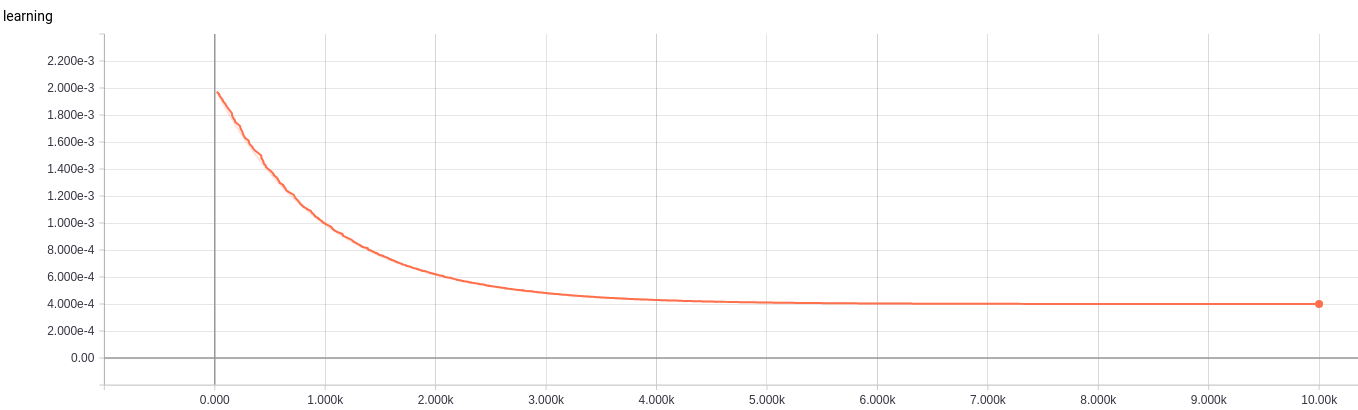
\includegraphics[width=\textwidth]{./images/learning_rate_localization.png}
                \caption{学习速率下降过程}
            \end{subfigure}
            
            \label{fig:confusion_matrix}
        \end{figure}

    \section{总结}

    (1)损失函数为课件示例中给出的SmoothL1 Loss(将对每个样本求和改为求均值),训练采用了Adam优化器。(2)实验中,仍然采用了按指数规律下降的学习速率。(3)使用tensorboard可以观测到loss的下降过程。(4)图像输入模型前经过了预处理,resize为224x224,并进行归一化。(5)考虑到显存大小,实验中batch大小取50。

\end{document}